\chapter{Introduction}

A \textit{compiler}
  converts from one representation
  to another.
A classic example
  is the GNU C Compiler, gcc, which
  compiles program written in C
  into low-level, processor-specific
  machine code,
  ready to be executed:
\begin{figure}[!h]
\centering
\begin{tikzpicture}
  \draw[inner sep = 5pt] (0,0) node [draw, thin] (c) \bgroup%
\begin{minipage}{10em}
\begin{minted}[fontsize=\small,baselinestretch=1]{c}
int square(int num) {
    return num * num;
}
\end{minted}
\end{minipage}
  \egroup;
  
\draw[inner sep = 5pt] (8.75,0) node [draw, thin] (asm) \bgroup%
\begin{minipage}{7em}
\begin{minted}[fontsize=\small,baselinestretch=1]{asm}
square:
 imul edi, edi
 mov eax, edi
 ret
\end{minted}
\end{minipage}
  \egroup;

\draw[inner sep = 5pt] (4.5,0) node [draw, thin] (compiler) {compiler};

  \draw[->, very thick] (c) edge (compiler) (compiler) edge (asm);
\end{tikzpicture}
\end{figure}

\noindent
We call the platform
  which the compiler is compiling for
  the \textit{target.}
% Inside a compiler are many processes,
%   only some of which relate to the the target:
% 
% \begin{figure}[h!]
%     \centering
% \begin{tikzpicture}
% \draw[inner sep = 5pt] (4.5,0) node [draw, thin] (compiler) {compiler};
% \draw (0,-2) node [draw,thin] (parser) {parser};
% \draw (compiler) edge (parser);
% \end{tikzpicture}
%     \label{fig:enter-label}
% \end{figure}
% 
\hl{diagram blowing up the compiler box?}
Though compilers perform many target-agnostic
  transformations and optimizations---%
  that is, modifications of the high-level code
  which are useful regardless of the target---%
  a compiler's most basic purpose
  is target-specific: that is,
  producing a program
  in the target's representation.
We call the target-specific portion
  of the compiler
  which implements this process
  a \textit{compiler backend,}
  and they will be the focus of this thesis.
  
Built in to every compiler backend
  is at least one model
  of the target platform.
These models come in all shapes
  and sizes.
For example,
  the x86 backend for gcc
  (that is, the portion of the compiler
    that compiles code for x86 processors)
  must understand
  the instructions available
  for x86;
  this is essentially a model
  of the x86 ISA.
\hl{get concrete examples here}
A compiler for deep learning
  workloads,
  on the other hand,
  must understand
  the potentially multiple
  available hardware accelerators,
  comprising a model
  of the system topology.

A compiler backend's
  internal hardware models
  are generally
  \textbf{implicit.}
That is, 
  the models are encoded in subtle ways;
  it would take an expert
  staring at the code
  to understand what the underlying hardware
  architecture
  actually is.
For example, \hl{example.}
  
Though they are the norm,
  implicit, handwritten hardware models
  present in a compiler
  are a problem
  for a number of reasons.
First, implicit, handwritten models
  are a great source of bugs.
Second, they are hard to change.
And third, 
  they leave potential optimizations
  on the table.

Implicit,
  handwritten models
  are a great source of bugs.
If your intention is to build a model
  of your underlying system,
  it is very easy to make a mistake
  while implementing that model,
  whether it be missing functionality,
  or misrepresenting the functionality
  of the hardware.
Furthermore, it is even easier
  to generate bugs
  (and harder to find them)
  when the model is implicit.

Implicit, handwritten models
  are also
  hard to build and change,
  and make compilers less extensible overall.
If every architecture is added
  by hand, manually,
  it discourages adding new ones.
If models are implicit
  and hard to understand,


Finally,
  implicit, handwritten models
  leave potential optimizations on the table.
\hl{would be nice to show that automated methods have clearly shown
  to be superior when it comes to optimizing programs.
  STOKE, AutoTVM, synthesis in general, ML guided?}

\textbf{Explicit} models of hardware,
  on the other hand,
  are not only pervasive,
  but are also prime for use with automated reasoning tools,
  in addition to often being more correct.
  
The reliance of modern compilers
  on \textit{implicit} models is truly odd, 
  given that
  explicit, formal models
  of the target hardware
  almost certainly exist
  in all cases.
In fact, nearly all hardware design
  \textit{begins} from the construction
  of these models
  at a high level of abstraction;
  the bulk of the hardware design process
  is building low-level implementations
  of the high-level specification,
  and verifying the implementation
  is equivalent.
Thus, \textbf{there is wealth
  of explicit, formal models of hardware
  which could be used
  instead of implicit models.}
\hl{examples of explicit hw models? alistair's work?
should probably go into a later paragraph}
\hl{maybe something about declarative programming being good?
a trend towards declarative programming?}

Furthermore, 
  there exist plenty of automated
  tools
  which deal with
  these formal models.
Oddly, though,
  many of these tools
  are concerned only with
  what happens \textit{after}
  compilation.
\hl{cite zach sisco latte, he says this directly}
That is, the formal models
  of hardware
  are used to check that 
  the compiled program is correct.
Why not instead
  just ensure
  that you can't compile an incorrect
  program?

Lastly, and perhaps most importantly,
  these explicit models
  are perhaps \textit{more correct}
  than any implicit, handwritten models
  that could be written,
  as in many cases, these models
  are the \textit{ground truth.}

Automated reasoning tools
  are ready for the challenge
  of automated compiler generation.

Finally, this leads to my thesis statement:

In this thesis,
  I present the case for
  automatically generating compiler backends
  from
  formal models of hardware.
I apply this technique
  to two separate domains:
  (1) compilation for
  domain-specific 
  deep learning accelerators,
  and
  (2) hardware compilation 
  (or \textit{synthesis})
  for Field-Programmable
  Gate Arrays (FPGAs).
In both of these cases,
  I show how
  automatically generating
  a portion of the compiler backend
  leads to increased correctness,
  greater extensibility,
  and more powerful automated optimization.

In the first part,
  I demonstrate
  how explicit,
  handwritten
  models of hardware,
  captured as
  \textit{rewrites,}
  can be used 
  to automatically implement
  ``instruction selection''
  for machine learning
  accelerators.

In the second part,
  I apply this thesis
  even more literally, by using
  formal models of hardware
  not written by us,
  but found in the wild,
  to build a compiler
  which automatically knows
  how to map designs
  to FPGAs.

The primary contributions of this dissertation
  are
\begin{itemize}
    \item blah
\end{itemize}
  
  

\section{Argument Structure}

This section outlines the hierarchical
  argument
  of this dissertation.
At the top is the 
  thesis of the dissertation;
  everything else present
  in this dissertation
  is meant to prove this thesis.
The next level of bullets
  represent the arguments
  which directly support this thesis.
Following from this,
  each subsequent level of bullets
  represent the arguments
  which support the previous level of
  arguments.
We use the symbol ``$\Leftarrow$''
  to capture the fact that
  each sublevel of arguments
  taken together
  should imply their parent claim.
  
  

\textbf{Thesis:}
  Automatically generating
  compiler backends
  from formal models of hardware
  improves correctness,
  leads to emergent optimization,
  and increases extensibility.
\begin{itemize}[label=$\Leftarrow$]
 \item Generating the backend
      for a compiler for deep learning
      accelerators
      by modeling hardware
      as rewrite rules
      leads to
      emergent optimizations
      and more mapping opportunities.
 \begin{itemize}[label=$\Leftarrow$]
  \item blah
 \end{itemize}
 \item Generating an FPGA technology
   mapper
   using semantics
   automatically extracted
   from Verilog simulation models
   leads to greater correctness,
   completeness,
   and extensibility.
    \begin{itemize}
        \item The models already exist in the form of Verilog simulation models.
    \end{itemize}
\end{itemize}

\section{Roadmap}

How to read this thesis.

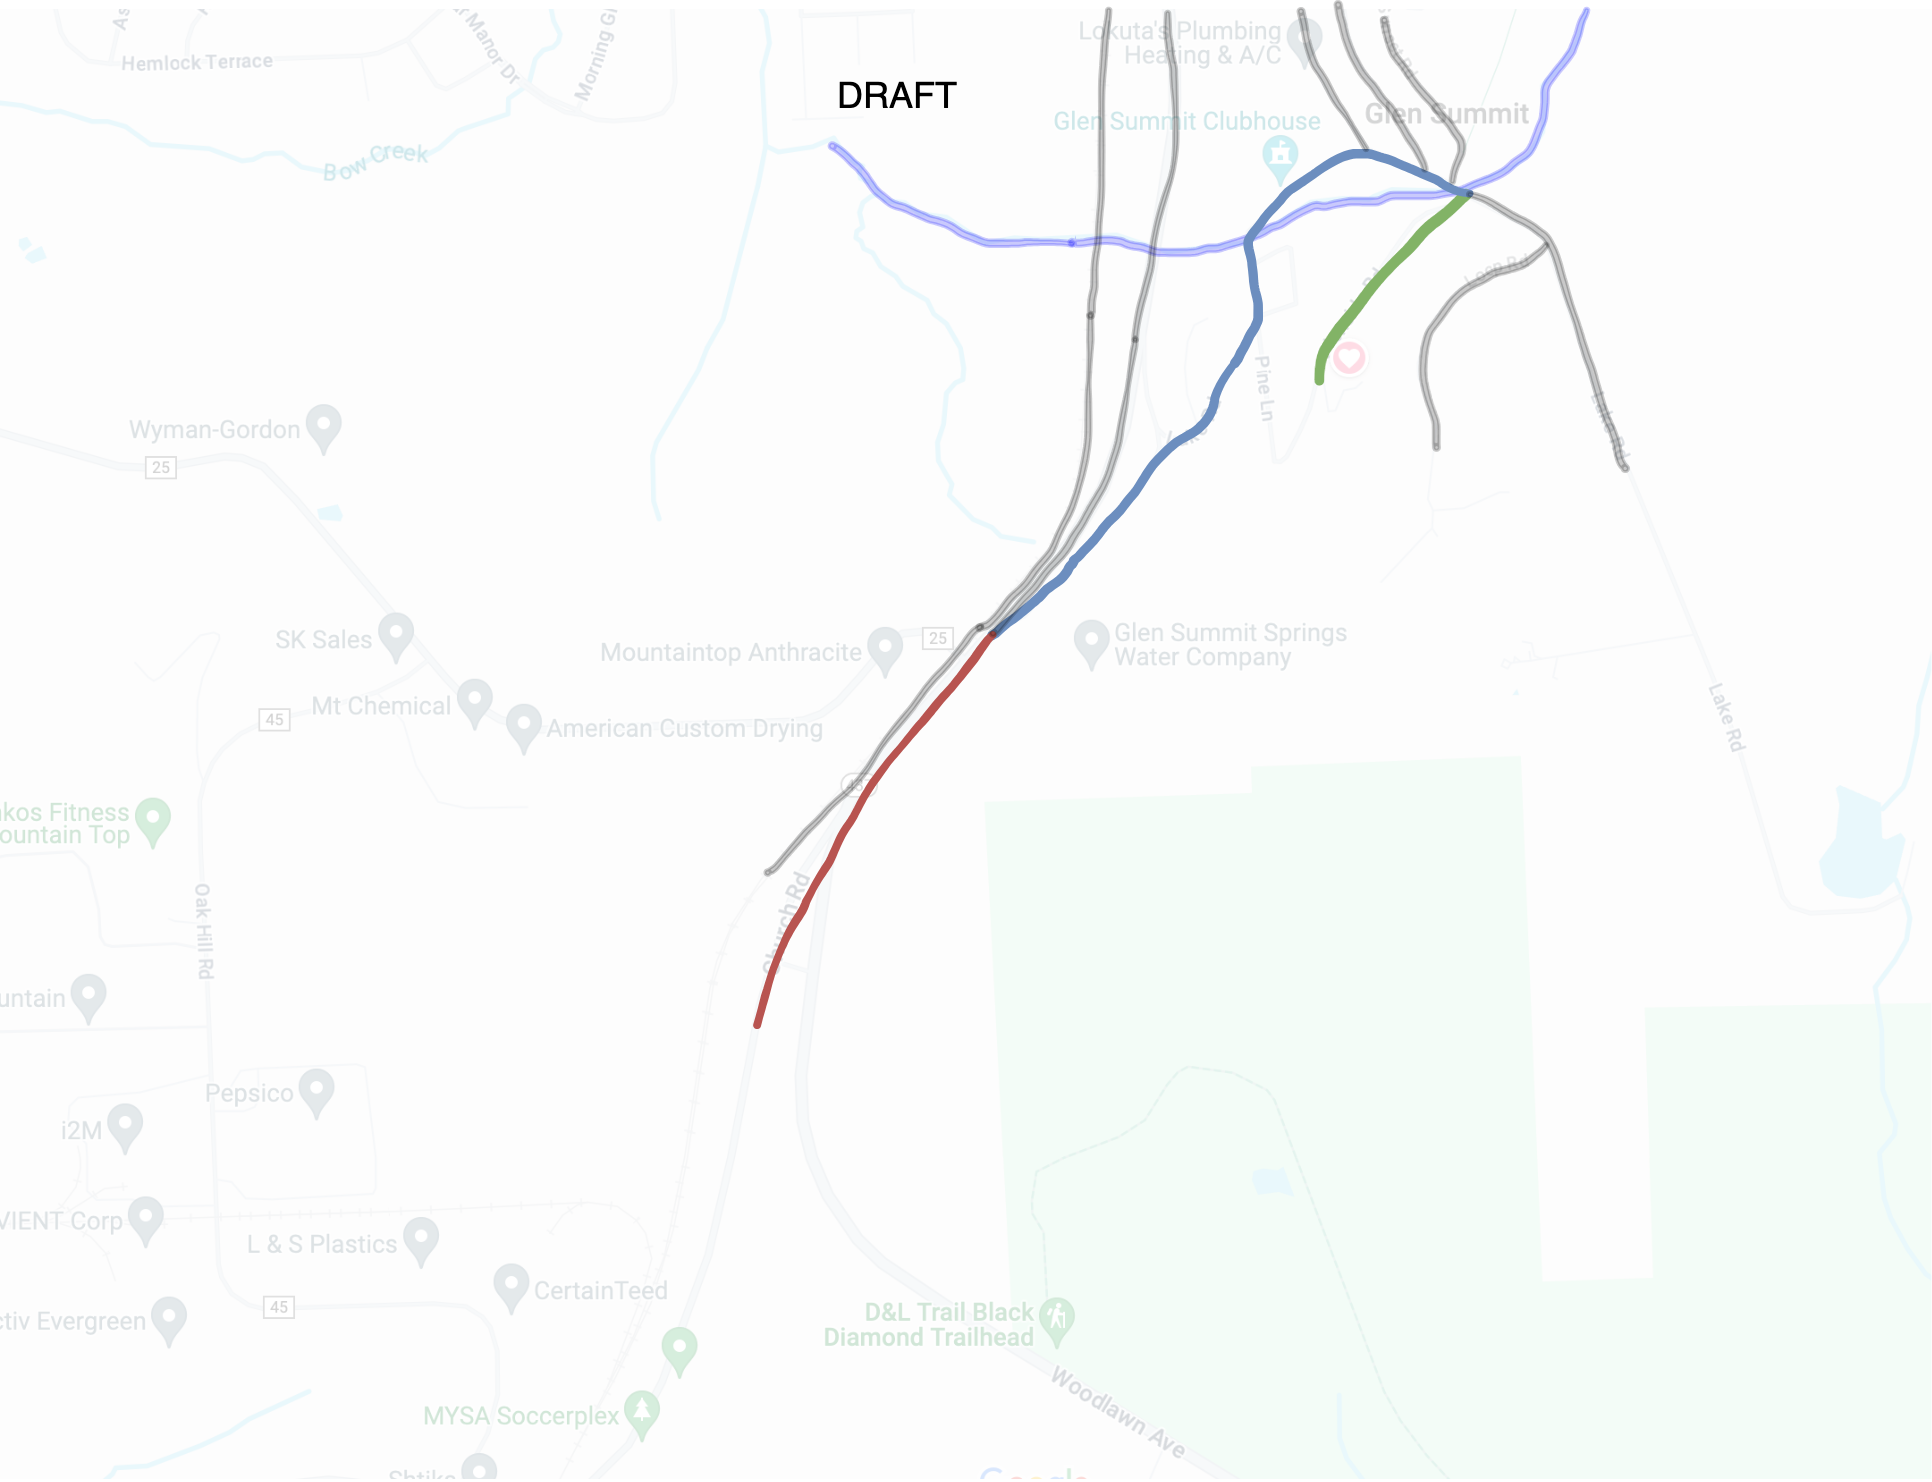
\includegraphics[width=\textwidth]{assets/street-diagram.drawio.png}